% Section 5, Training the Searcher.
\section{Training the Searcher}
\label{sec:training}

\subsection{Data and Supervised Training}
\label{sec:training-data}

\modelname is trained on search-phase demonstrations sliced from openly licensed
agent trajectories produced by other systems. Each demonstration captures one
complete search episode: the agent explores a repository, localizes the fault,
and writes a failing reproduction, with a synthesized handoff-emission turn
appended as the final supervised target. Within that synthesized turn, the
file list is extracted deterministically from the trace and the reproduction
record is copied verbatim; only the free-form notes are written by a model,
the open-weights gpt-oss-120b~\citep{gptoss}. Traces are drawn from three public
sources (\dataset{Open-SWE-Traces}~\citep{openswetraces},
\dataset{SWE-rebench-openhands}~\citep{nebiusrebench,swerebench}, and
\dataset{SWE-Hero}~\citep{swehero}; the latter two are trajectories of
the OpenHands scaffold~\citep{openhands}) and then success-filtered
against the gold patch, keeping only trajectories that actually found the right files.
Deduplication retains the two highest quality-ranked traces per issue, so the
corpus counts distinct bugs rather than retellings of the same fix.

The resulting dataset contains 19{,}911 examples. Six rows carrying malformed
tool-call wrappers are dropped at load time, giving the 19{,}905 examples
actually trained on. The realized language mix is Python 37.3\%, Go 36.7\%,
TypeScript 19.7\%, and JavaScript 6.3\%.
Table~\ref{tab:training-data} summarizes the corpus composition.

\begin{table}[!tbp]
\centering
\caption{\textbf{Composition of \modelname's supervised search corpus.}
Each example is a full search trajectory with a synthesized
handoff-emission turn as the final supervised step; loss is on assistant
turns only.  Traces are success-filtered and deduplicated to two per
issue.  The 23 evaluation repositories and 450 held-out vault issues are
excluded; both exclusions were verified by a programmatic gate.}
\label{tab:training-data}
% ===========================================================================
% tab-training-data.tex — composition of the frozen \modelname SFT set (§5).
% BODY ONLY (tabular). Wrapper/caption/label live in the section file.
%
% PROVENANCE — every cell. All numbers are the REALIZED built set, not the
% planning targets; where the two differ the divergence is stated below.
%
%   COUNTS
%     19,911 = the frozen dataset as built and pushed.
%       internal records, "Final counts": "Set: 19,911
%       (size preserved) - Shelf: 9,478"; internal records
%       "SFT DATASET FROZEN: sft_set_clean.jsonl final (19,911 ...)".
%     19,905 = the EFFECTIVE training count, and the number this table
%       reports as "examples trained on". Two load-time drops were applied
%       after the freeze, both deliberate, both leaving the HF file
%       untouched:
%         internal records: "malformed 9 rows ... drop 3 phantom-tool
%         rows -> 19,908 at load";
%         internal records: 3 further rows carrying a stray off-dialect
%         tool-call wrapper dropped at load -> "Effective training count
%         19,905. HF file untouched."
%       Independently confirmed by the run's own dataset fingerprint,
%       internal records: "Run identity": "dataset_hash: 87762bd2f14b
%       (fp 2f0092f6373a2882 - 12,723 blocks / 19,905 ex / 382,417,805 tok /
%       91.7% fill)".
%     Shelf 9,478 = internal records, same line (the 3rd-best trace per
%       bug, held as an underfit lever; NEVER trained on).
%
%   LANGUAGE MIX — realized, from internal records "Language
%   mix (unchanged)": Go 7,304 (36.7%) - Python 7,417 (37.3%) - TypeScript
%   3,932 (19.7%) - JavaScript 1,258 (6.3%). The same four percentages
%   appear in internal records.
%     DIVERGENCE FROM PLAN (stated, not silently reconciled): the target in
%     internal records is "Language mix ~ Pro: ~38% Go / 36% Py / 25%
%     TS-JS". The realized set is 36.7 / 37.3 / 26.0 (TS+JS) --- close, and
%     internal records report "Residual Go loss: ZERO net loss", so the Go
%     shortfall never bit. This table prints the REALIZED numbers.
%     The counts sum over the 19,911-example built set; the 6 load-time
%     drops are not attributed to a language in any source, so percentages
%     are quoted against 19,911 exactly as the source computes them.
%
%   SOURCE DATASETS — internal records ("Sources: Open-SWE-Traces
%   (primary; only Go/TS source; blocklist-CLEAN) - nebius-rebench-openhands
%   - SWE-Hero (filter 73 rows)") and internal records,
%   which names them nvidia/Open-SWE-Traces (207,489 trajectories),
%   nebius/SWE-rebench-openhands (67,074, Python), nvidia/SWE-Hero-openhands
%   (34,269, Python) and states "Open-SWE-Traces is the load-bearing source
%   --- the only one with Go/TS/JS. nebius + SWE-Hero are Python top-ups".
%   Per-source example counts in the FINAL set are not broken out in any
%   frozen document, so this table names the sources and their roles and
%   does not invent a per-source split.
%     A per-source example count for the final 19,905 is not recorded
%     anywhere; one would have to be recomputed from the frozen set.
%
%   DEDUP RULE — internal records: "per issue keep the
%   2 best successful traces, quality-ranked (repro present > efficient >
%   shortest; source-model diversity as tiebreak); 3rd-best trace saved as
%   the named 'shelf'". Ratified internally ("2 best
%   traces per bug (~21k demos; 2v3 adds retellings, not distinct bugs)").
%
%   BLOCKLIST — internal records: "The 23-repo blocklist (excluded from
%   ALL training/RL/label data)": Pro-11 (ansible/ansible,
%   internetarchive/openlibrary, flipt-io/flipt, qutebrowser/qutebrowser,
%   gravitational/teleport, protonmail/webclients, future-architect/vuls,
%   navidrome/navidrome, element-hq/element-web, NodeBB/NodeBB,
%   tutao/tutanota) + Verified-12 (astropy, django, matplotlib, seaborn,
%   flask, requests, xarray, pylint, pytest, scikit-learn, sphinx, sympy).
%   Enforcement measured, not asserted: internal records, "Sanity gate ---
%   PASSED": "0 vault hits - 0 blocklist hits".
%
%   HELD-OUT VAULT — 450 issues (Go 200 / TS 150 / Py 100, 306 repos),
%   internal records ("Held-out vault BUILT ... vault IDs = mandatory
%   exclusion list for all training sets"). Also 0 hits at the gate.
%
%   REPRO VALIDITY — internal records: "Repro-validity: 84.9% -> 97.67%
%   (464/19,911 false, all Go)"; the 464 are kept with honest
%   reproduced:false labels (internal ruling).
%
%   TOKENS / PACKING — internal records, "Run identity" (same fingerprint):
%   382,417,805 tokens per epoch packed into 12,723 blocks of 32k at 91.7%
%   fill.
% ===========================================================================
\begin{tabular}{@{}lr@{}}
\toprule
Component & Value \\
\midrule
\multicolumn{2}{@{}l}{\emph{Corpus}} \\
Examples trained on          & 19,905 \\
Built / frozen set           & 19,911 \\
Held-back shelf (untrained)  & 9,478 \\
Tokens per epoch             & 382.4M \\
Packed 32k blocks (fill)     & 12,723 (91.7\%) \\
\midrule
\multicolumn{2}{@{}l}{\emph{Language mix}} \\
Go                           & 7,304 (36.7\%) \\
Python                       & 7,417 (37.3\%) \\
TypeScript                   & 3,932 (19.7\%) \\
JavaScript                   & 1,258 \phantom{0}(6.3\%) \\
\midrule
\multicolumn{2}{@{}l}{\emph{Trace sources}} \\
Open-SWE-Traces              & Go/TS/JS + Py \\
SWE-rebench-openhands        & Python \\
SWE-Hero-openhands           & Python \\
\midrule
\multicolumn{2}{@{}l}{\emph{Filters}} \\
Traces kept per issue        & top 2 \\
Verified reproduction        & 97.7\% \\
Excluded repositories        & 23 \\
Excluded held-out issues     & 450 \\
\bottomrule
\end{tabular}

\end{table}

Contamination control was decided on day one: a 23-repository blocklist
covering all 11 SWE-bench Pro repositories and 12 SWE-bench
Verified~\citep{swebenchverified} repositories is excluded from every
training and calibration set. A
programmatic gate verified zero blocklist hits in the frozen file.

We fine-tune Qwen2.5-Coder-7B~\citep{qwen25coder} with
LoRA~\citep{lora} on a single GPU. Before training, the base model's
localization rate is near zero; the search behavior is entirely learned from
the demonstrations above. Hyperparameters are reported in Appendix~\ref{apx:hyperparams}.

\subsection{Decoding Matters More Than Expected}
\label{sec:decoding}

The most consequential training-era finding was not about the training itself
but about inference. On a 450-task held-out exam, greedy decoding finds the
right files at a rate of 0.1104. A single sampled draw at temperature 0.9
reaches 0.3058, a 2.65$\times$ gain after matching for infrastructure timeouts.

\begin{figure}[!tbp]
% ===========================================================================
% fig-decoding.tex — the sampled-decoding discovery, two panels.
% BODY ONLY (tikzpicture). Wrapper/caption/label live in the section file.
% Requires % ===========================================================================
% fig-style.tex — shared colour / marker scheme for EVERY main-paper figure.
% \input this ONCE from the preamble of main.tex (after tikz + pgfplots).
%
% House rule: the palette is defined here and nowhere else. Each series also
% gets a distinct marker AND line style so the figures survive grayscale
% printing.
%
%   \sysname / deployed .. cSys   (blue!70!black)    mark *
%   opus / claude ........ cOpus  (red!70!black)     mark square*
%   gpt .................. cGpt   (teal!70!black)    mark triangle*
%   kimi ................. cKimi  (violet!70!black)  mark diamond*
%   flash ................ cFlash (orange!70!black)  mark pentagon*
%   greedy / baseline .... cBase  (gray)             mark o
% ===========================================================================
% The pipeline diagram needs the calc library for coordinate arithmetic; the
% rest of the libraries are already loaded in main.tex's preamble.
\usetikzlibrary{calc}
% Hatching, so bar charts stay readable in grayscale.
\usetikzlibrary{patterns}

\colorlet{cSys}{blue!70!black}
\colorlet{cOpus}{red!70!black}
\colorlet{cGpt}{teal!70!black}
\colorlet{cKimi}{violet!70!black}
\colorlet{cFlash}{orange!70!black}
\colorlet{cBase}{gray}

% Common axis furniture: footnotesize ticks/legend, small titles, framed
% legend in gray!50, light horizontal grid.
\pgfplotsset{
  paperaxis/.style={
    width=0.80\linewidth,
    height=5.2cm,
    tick label style={font=\footnotesize},
    label style={font=\footnotesize},
    title style={font=\small},
    legend style={font=\footnotesize, draw=gray!50, fill=white,
                  fill opacity=0.9, text opacity=1, rounded corners=1pt},
    every axis plot/.append style={line width=0.7pt},
    grid style={gray!25, line width=0.3pt},
    axis line style={gray!60},
    tick style={gray!60},
  },
  papermark/.style={mark size=2.6pt},
}
 in the preamble.
%
% PROVENANCE — every number.
%   PANEL 1 (450-task vault). Source: internal records, header table
%     "450-VAULT MILESTONE — merged-e2.0 —
%     run A (temp 0.9) vs run B (greedy)", row `find_rate`:
%       RUN B (greedy)   0.1104
%       RUN A (temp 0.9) 0.3058
%     n = 450 per arm (row `n`).
%     Multiplier: the same source's timeout-sensitivity section —
%       RAW      A=0.3058 B=0.1104  ratio 2.77x
%       MATCHED  A=0.3091 B=0.1166  ratio 2.65x  (n=426)
%     The LICENSED multiplier is the timeout-matched 2.65x, which is what is
%     annotated on the panel.
%     *** Never quote a 5.7x multiplier anywhere: that figure's denominator
%     was a prefix-cache-contaminated run. ***
%
%   PANEL 2 (100-task dial subset — a DIFFERENT task set from panel 1).
%     Source: internal records, the decomposition of where the gain comes
%     from:
%       "commit rate 3.03x  x  per-handoff quality 0.96x  =  find-rate 2.91x"
%     Underlying per-handoff recall: greedy 0.526 vs temp 0.9 0.505 (same
%     section); commit/handoff coverage 0.2367 -> 0.7167 (CHECK 2 table).
%     Task set = dial_subset_100 (md5 cb363beb...), 300 episodes per arm
%     (3 replicates x 100), per CHECK 1 / CHECK 2 tables.
% ===========================================================================
\begin{tikzpicture}
\begin{groupplot}[
  paperaxis,
  group style={
    group size=2 by 1,
    horizontal sep=13mm,
  },
  width=0.44\linewidth,
  height=5.0cm,
  xticklabel style={font=\footnotesize},
  ymajorgrids=true,
  enlarge x limits=0.55,
  nodes near coords,
  nodes near coords style={font=\scriptsize, color=black},
]

% ---- PANEL 1: find rate, vault-450 -------------------------------------
\nextgroupplot[
  ybar, bar width=11pt,
  title={Find rate (vault-450)},
  ylabel={Mean gold-file recall},
  ymin=0, ymax=0.40,
  ytick={0,0.1,0.2,0.3,0.4},
  symbolic x coords={greedy,{temp 0.9}},
  xtick={greedy,{temp 0.9}},
  nodes near coords={\pgfmathprintnumber[fixed, fixed zerofill, precision=3]{\pgfplotspointmeta}},
]
\addplot[fill=cBase!45, draw=cBase!80!black, bar shift=0pt]
  coordinates {(greedy,0.1104)};
\addplot[fill=cSys!35, draw=cSys, bar shift=0pt,
         postaction={pattern=north east lines, pattern color=cSys!45}]
  coordinates {({temp 0.9},0.3058)};
\node[font=\scriptsize, anchor=south, align=center, text=cSys!80!black]
  at (axis cs:greedy,0.20) {$2.65\times$\\timeout-\\matched};

% ---- PANEL 2: decomposition, 100-task dial subset ----------------------
\nextgroupplot[
  ybar, bar width=11pt,
  title={Decomposition (dial-100)},
  ylabel={Ratio, temp 0.9 $/$ greedy},
  ymin=0, ymax=3.9,
  ytick={0,1,2,3},
  symbolic x coords={{commit rate},{per-handoff}},
  xtick={{commit rate},{per-handoff}},
  xticklabels={commit\\rate, handoff\\quality},
  xticklabel style={font=\scriptsize, align=center},
  nodes near coords={$\pgfmathprintnumber[fixed, precision=2]{\pgfplotspointmeta}\times$},
]
\addplot[fill=cSys!35, draw=cSys, bar shift=0pt]
  coordinates {({commit rate},3.03)};
\addplot[fill=cBase!45, draw=cBase!80!black, bar shift=0pt]
  coordinates {({per-handoff},0.96)};
% parity line at ratio 1.0; ymin=0, ymax=3.9 -> axis fraction 1/3.9.
\draw[dashed, gray!70, line width=0.6pt]
  (rel axis cs:0,0.25641) -- (rel axis cs:1,0.25641);
\node[font=\scriptsize, anchor=south west, text=gray!60!black]
  at (rel axis cs:0.03,0.29) {parity};

\end{groupplot}
\end{tikzpicture}

\caption{\textbf{Sampled decoding is what makes the searcher useful.}
\textbf{Left:} switching from greedy to temperature $0.9$ raises the
find rate from $0.110$ to $0.306$ ($2.65\times$, $n{=}426$ of $450$).
\textbf{Right:} on a separate 100-task dial set, commitment rises
$3.03\times$ while per-handoff quality holds at $0.96\times$; on the
exam itself emission rises $3.4\times$ against an 18\% per-handoff
recall cost (Appendix~\ref{apx:vault}).  The two panels use different
task sets; the right panel is a mechanism check, not a replication.}
\label{fig:decoding}
\end{figure}

The exam's own decomposition shows what sampling buys and what it
spends: the searcher's emission rate rises from 0.213 to 0.718
(3.4$\times$), while recall per emitted handoff falls from 0.517 to
0.426, an 18\% quality cost (Appendix~\ref{apx:vault}). Sampling trades
a slice of per-handoff quality for a much larger gain in willingness to
commit, a strongly net-positive exchange. A separate 100-task dial set
shows the same mechanism with commitment up 3.03$\times$ and per-handoff
quality flat at 0.96$\times$ (Figure~\ref{fig:decoding}); the quality
cost visible on the exam does not appear there, so the dial set is a
mechanism check, not a replication. Greedy decoding, it turns out,
makes the searcher reluctant to declare a result; sampling at moderate
temperature recovers ability the model already has. The shipped
configuration is therefore a single sampled draw at temperature 0.9
(\S\ref{sec:setup}).

\subsection{Language Transfer}
\label{sec:language-transfer}

\modelname is trained on four languages (Go, Python, TypeScript, JavaScript),
yet \sysname is deployed against repositories in languages the searcher has
never seen. On the nine-language SWE-bench Multilingual
evaluation~\citep{swebenchmultilingual}, which contains no Python and so
covers three of the four training languages
(Figure~\ref{fig:language-transfer}), spontaneous-handoff localization quality
is higher on the six never-trained languages (file-level $F_1 = 0.630$) than on
the three trained ones ($F_1 = 0.455$). The inversion survives a
difficulty-matched control restricted to single-gold-file tasks, where recall
on never-trained languages reaches 0.791 versus 0.524 for the trained pool.
JavaScript and TypeScript account for much of the trained pool's lower average;
the TypeScript and C++ cells each rest on 12 assigned tasks, of which 7 and 8
respectively produced the spontaneous handoffs analyzed, and are indicative
only (full per-language table in Appendix~\ref{apx:languages}).

\begin{figure}[!tbp]
% ===========================================================================
% fig-language-transfer.tex — per-language spontaneous localization F1,
% trained vs never-trained languages.
% BODY ONLY (tikzpicture). Wrapper/caption/label live in the section file.
% Requires % ===========================================================================
% fig-style.tex — shared colour / marker scheme for EVERY main-paper figure.
% \input this ONCE from the preamble of main.tex (after tikz + pgfplots).
%
% House rule: the palette is defined here and nowhere else. Each series also
% gets a distinct marker AND line style so the figures survive grayscale
% printing.
%
%   \sysname / deployed .. cSys   (blue!70!black)    mark *
%   opus / claude ........ cOpus  (red!70!black)     mark square*
%   gpt .................. cGpt   (teal!70!black)    mark triangle*
%   kimi ................. cKimi  (violet!70!black)  mark diamond*
%   flash ................ cFlash (orange!70!black)  mark pentagon*
%   greedy / baseline .... cBase  (gray)             mark o
% ===========================================================================
% The pipeline diagram needs the calc library for coordinate arithmetic; the
% rest of the libraries are already loaded in main.tex's preamble.
\usetikzlibrary{calc}
% Hatching, so bar charts stay readable in grayscale.
\usetikzlibrary{patterns}

\colorlet{cSys}{blue!70!black}
\colorlet{cOpus}{red!70!black}
\colorlet{cGpt}{teal!70!black}
\colorlet{cKimi}{violet!70!black}
\colorlet{cFlash}{orange!70!black}
\colorlet{cBase}{gray}

% Common axis furniture: footnotesize ticks/legend, small titles, framed
% legend in gray!50, light horizontal grid.
\pgfplotsset{
  paperaxis/.style={
    width=0.80\linewidth,
    height=5.2cm,
    tick label style={font=\footnotesize},
    label style={font=\footnotesize},
    title style={font=\small},
    legend style={font=\footnotesize, draw=gray!50, fill=white,
                  fill opacity=0.9, text opacity=1, rounded corners=1pt},
    every axis plot/.append style={line width=0.7pt},
    grid style={gray!25, line width=0.3pt},
    axis line style={gray!60},
    tick style={gray!60},
  },
  papermark/.style={mark size=2.6pt},
}
 in the preamble.
%
% PROVENANCE — every number.
%   Source: internal records (run-4 handoff quality,
%   SWE-bench Multilingual, single draw @ temp 0.9, solo searcher, no fixer
%   in the loop).
%
%   Per-language bars = per-language file quality against gold-PATCH files,
%   column "SPONT P / R / F1", F1 component only:
%     Go          trained  0.546   (spont n=27, total n=42)
%     JavaScript  trained  0.389   (spont n=26, total n=31)
%     TypeScript  trained  0.343   (spont n=7,  total n=12)  *indicative
%     Java        never    0.612   (spont n=27, total n=43)
%     Ruby        never    0.701   (spont n=36, total n=44)
%     Rust        never    0.667   (spont n=20, total n=43)
%     PHP         never    0.630   (spont n=33, total n=42)
%     C           never    0.435   (spont n=18, total n=30)
%     C++         never    0.708   (spont n=8,  total n=12)  *indicative
%
%   Aggregate reference lines = trained vs never-trained aggregate,
%   spontaneous arm:
%     trained (Go/JS/TS)                     n=60  F1 0.455
%     never-trained (Java/Ruby/Rust/PHP/C/C++) n=142 F1 0.630
%
%   Pools: trained = Go, JavaScript, TypeScript
%   (Python is absent from the training pool); never-trained = Java, Ruby,
%   Rust, PHP, C, C++.
%   Indicative-only flag for TypeScript (n=12) and C++ (n=12) = the report's
%   own binding stamp.
%   Spontaneous and forced handoffs are NEVER pooled; only the spontaneous
%   arm is plotted here.
% ===========================================================================
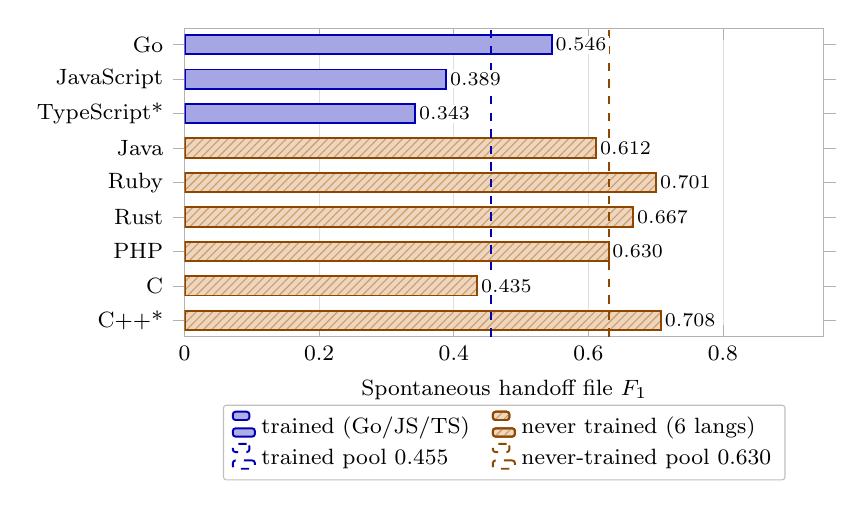
\begin{tikzpicture}
\begin{axis}[
  paperaxis,
  width=0.80\linewidth,
  height=5.5cm,
  xbar,
  bar width=7pt,
  xmin=0, xmax=0.95,
  xtick={0,0.2,0.4,0.6,0.8},
  xlabel={Spontaneous handoff file $F_1$},
  symbolic y coords={{Go},{JavaScript},{TypeScript*},
                     {Java},{Ruby},{Rust},{PHP},{C},{C++*}},
  ytick={{Go},{JavaScript},{TypeScript*},
         {Java},{Ruby},{Rust},{PHP},{C},{C++*}},
  y dir=reverse,
  enlarge y limits=0.06,
  xmajorgrids=true,
  nodes near coords,
  % white fill so the two dashed pool lines never run through a value label
  nodes near coords style={font=\scriptsize, fill=white, inner sep=1pt,
                           /pgf/number format/fixed,
                           /pgf/number format/fixed zerofill,
                           /pgf/number format/precision=3},
  legend style={at={(0.5,-0.22)}, anchor=north, legend columns=2,
                /tikz/every even column/.append style={column sep=6pt}},
  legend cell align=left,
]

% ---- trained pool: Go / JavaScript / TypeScript (solid) ----------------
\addplot[fill=cSys!35, draw=cSys, bar shift=0pt]
  coordinates {(0.546,{Go}) (0.389,{JavaScript}) (0.343,{TypeScript*})};
\addlegendentry{trained (Go/JS/TS)}

% ---- never-trained pool (hatched, so the split survives grayscale) -----
\addplot[fill=cFlash!25, draw=cFlash!80!black, bar shift=0pt,
         postaction={pattern=north east lines, pattern color=cFlash!60}]
  coordinates {(0.612,{Java}) (0.701,{Ruby}) (0.667,{Rust})
               (0.630,{PHP}) (0.435,{C}) (0.708,{C++*})};
\addlegendentry{never trained (6 langs)}

% ---- pooled aggregates: 0.455 (trained) and 0.630 (never-trained) ------
% x positions as axis fractions: 0.455/0.95 and 0.630/0.95.
\draw[dashed, cSys, line width=0.7pt]
  (rel axis cs:0.47895,0) -- (rel axis cs:0.47895,1);
\draw[dashed, cFlash!80!black, line width=0.7pt]
  (rel axis cs:0.66316,0) -- (rel axis cs:0.66316,1);
% the two dashed lines are identified in the legend rather than in-plot,
% where they would collide with the bar value labels.
\addlegendimage{dashed, cSys, line width=0.7pt}
\addlegendentry{trained pool 0.455}
\addlegendimage{dashed, cFlash!80!black, line width=0.7pt}
\addlegendentry{never-trained pool 0.630}

\end{axis}
\end{tikzpicture}

\caption{\textbf{Localization transfers to languages \modelname was never
trained on.}  Per-language file-level $F_1$ of spontaneous handoffs
(searcher alone, single draw, SWE-bench Multilingual).  Solid bars:
three trained languages; hatched: six never-trained.  Dashed lines mark
pooled aggregates ($0.455$ trained, $0.630$ never-trained).
The TypeScript and C++ cells (12 assigned tasks each; 7 and 8
spontaneous handoffs analyzed) are indicative only.}
\label{fig:language-transfer}
\end{figure}

The contrast carries a confound: JavaScript and TypeScript are at once the
trained pool's weakest cells and its smallest training slices, and both may be
structurally harder to localize in (dynamic imports, build artifacts)
independently of training exposure, so the trained-versus-never-trained
comparison should not be read as causal.
Our hypothesis for the pattern, and it is a hypothesis, is that \modelname
learned a search method, not a language-specific vocabulary. The exploration
strategies it relies on (reading directory trees, tracing imports, scanning
test files) are structural operations that generalize across languages; the
specific tokens involved matter less than the strategy of following them.

\medskip
\noindent\textbf{Reinforcement learning.}\quad
We built and validated a GRPO~\citep{grpo} training rig and ran 50 clean
steps. Learning was flat. A trace-level autopsy showed that the reward signal
was real but aimed at a behavior already near its ceiling after supervised
training: the model could localize when it chose to commit, and sampling had
already recovered that commitment. We shelved RL in favor of the decoding fix
described above; rig details are in Appendix~\ref{apx:hyperparams}.

\FloatBarrier
